\documentclass[class=article, crop=false]{standalone}
\usepackage{tikz}
\usepackage{subcaption}
\usetikzlibrary{calc}

\begin{document}
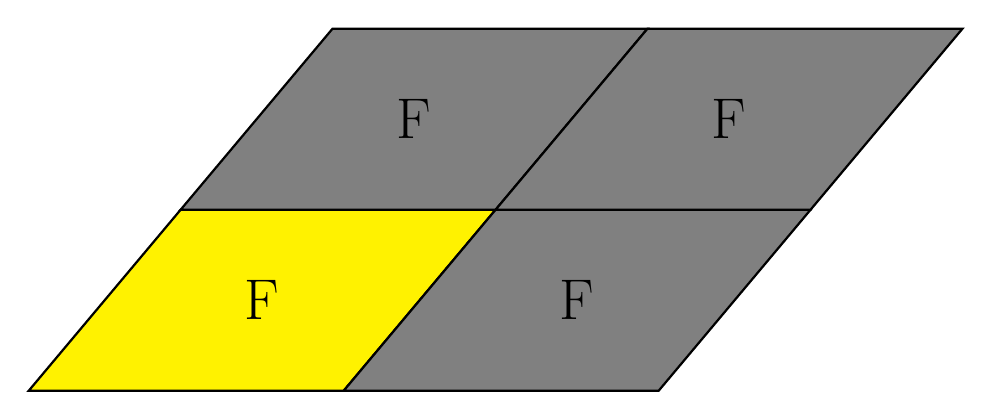
\begin{tikzpicture}
    % Define the lengths of the sides and the angle
    \def\a{4}  % length of side a
    \def\b{3}  % length of side b
    \def\angle{50}  % angle between sides a and b
    \def\s{F} % Label in center of cells

    % Calculate the coordinates of the points
    \coordinate (C00) at (0, 0);
    \coordinate (C10) at (\a, 0);
    \coordinate (C11) at ({\a + \b*cos(\angle)}, {\b * sin(\angle)});
    \coordinate (C01) at ({\b * cos(\angle)}, {\b * sin(\angle)});
    \coordinate (C02) at ({2*\b*cos(\angle)}, {2*\b * sin(\angle)});
    \coordinate (C12) at ({\a +2*\b * cos(\angle)}, {2*\b * sin(\angle)});
    \coordinate (C22) at ({2*\a + 2*\b * cos(\angle)}, {2*\b * sin(\angle)});
    \coordinate (C21) at ({2*\a + \b*cos(\angle)}, {\b * sin(\angle)});
    \coordinate (C20) at ({2*\a}, 0);

        
    % Draw the oblique unit cell
    \draw[thick,fill=yellow] (C00) -- (C10) -- (C11) -- (C01) -- cycle;
    \draw[thick,fill=gray] (C01) -- (C11) -- (C12) -- (C02) -- cycle;
    \draw[thick,fill=gray] (C10) -- (C20) -- (C21) -- (C11) -- cycle;
    \draw[thick,fill=gray] (C11) -- (C21) -- (C22) -- (C12) -- cycle;

    % Center symbols
    \node at ($(C00)!0.5!(C11)$) {\huge \s};
    \node at ($(C20)!0.5!(C11)$) {\huge \s};
    \node at ($(C02)!0.5!(C11)$) {\huge \s};
    \node at ($(C22)!0.5!(C11)$) {\huge \s};
\end{tikzpicture}
\end{document}